% generated by hydro.experiments.tikz; do not edit by hand
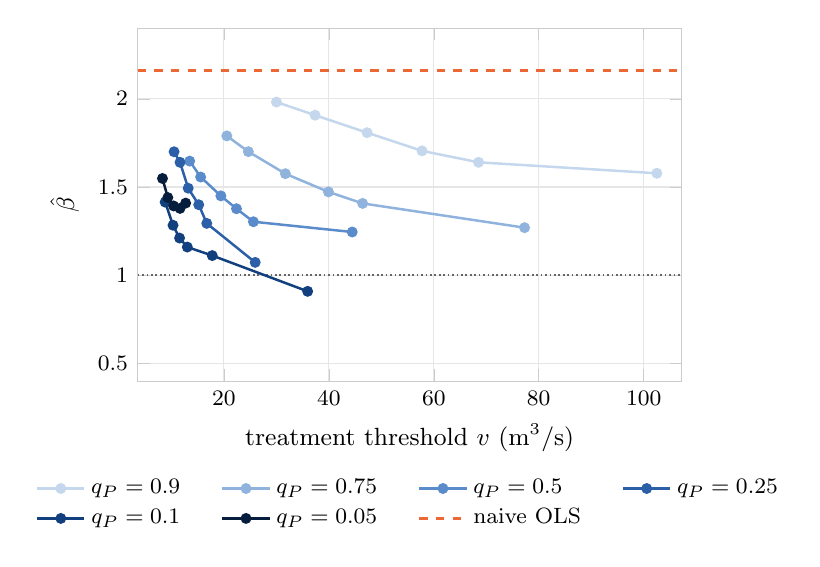
\begin{tikzpicture}
\definecolor{appblue}{HTML}{2A78D6}
\definecolor{apporange}{HTML}{EB6834}
\definecolor{appgreen}{HTML}{1BAF7A}
\definecolor{appviolet}{HTML}{4A3AA7}
\definecolor{appgrey}{HTML}{8A8A8A}
\definecolor{applight}{HTML}{CCCCCC}
\definecolor{appq0}{HTML}{C4D7EC}
\definecolor{appq1}{HTML}{8FB3DD}
\definecolor{appq2}{HTML}{5A8BCB}
\definecolor{appq3}{HTML}{2B5FA8}
\definecolor{appq4}{HTML}{123F7E}
\definecolor{appq5}{HTML}{061D3D}
\begin{axis}[
  width=0.7\textwidth, height=0.5\textwidth,
  ymin=0.4, ymax=2.4, ytick={0.5,1,1.5,2}, xtick={20,40,...,100}, enlarge x limits=0.05,
  xlabel={treatment threshold $v$ (m$^3$/s)}, ylabel={$\hat\beta$},
  xmajorgrids, ymajorgrids, grid style={applight!50}, axis line style={applight}, tick style={applight},
  tick label style={font=\footnotesize}, label style={font=\small},
  title style={font=\small, yshift=-3pt},
  every axis plot/.append style={line width=0.9pt, mark size=1.5pt},
  legend columns=4, legend style={at={(0.5,0)}, anchor=north, yshift=-1.1cm, draw=none, fill=none, font=\footnotesize, legend cell align=left,
  /tikz/every even column/.append style={column sep=0.45cm}},
  clip=false,
]
\draw[densely dotted, black!60, line width=0.6pt] ({rel axis cs:0,0}|-{axis cs:0,1.0}) -- ({rel axis cs:1,0}|-{axis cs:0,1.0});
\draw[dashed, apporange, line width=0.9pt] ({rel axis cs:0,0}|-{axis cs:0,2.1600}) -- ({rel axis cs:1,0}|-{axis cs:0,2.1600});
\addplot[appq0, mark=*] coordinates {(30.016,1.9815) (37.378,1.907) (47.289,1.8079) (57.766,1.7048) (68.527,1.64) (102.51,1.5778)};
\addlegendentry{$q_P = 0.9$}
\addplot[appq1, mark=*] coordinates {(20.558,1.7896) (24.664,1.7004) (31.715,1.5754) (39.927,1.4723) (46.44,1.407) (77.305,1.2695)};
\addlegendentry{$q_P = 0.75$}
\addplot[appq2, mark=*] coordinates {(13.479,1.6468) (15.574,1.5566) (19.425,1.4497) (22.399,1.3768) (25.627,1.3031) (44.457,1.2449)};
\addlegendentry{$q_P = 0.5$}
\addplot[appq3, mark=*] coordinates {(10.506,1.6998) (11.638,1.6399) (13.196,1.4931) (15.206,1.3995) (16.735,1.2938) (25.967,1.0727)};
\addlegendentry{$q_P = 0.25$}
\addplot[appq4, mark=*] coordinates {(8.8065,1.4142) (10.307,1.2832) (11.553,1.2106) (13.026,1.1596) (17.783,1.1113) (35.962,0.90854)};
\addlegendentry{$q_P = 0.1$}
\addplot[appq5, mark=*] coordinates {(8.2968,1.5483) (9.3162,1.4401) (10.421,1.3927) (11.638,1.3788) (12.714,1.4087)};
\addlegendentry{$q_P = 0.05$}
\addlegendimage{apporange, dashed}\addlegendentry{naive OLS}
\end{axis}
\end{tikzpicture}
